% !TEX root = main.tex
\section{Results}\label{results}

\subsection{Overview of Results}\label{overview-of-results}

This section reports (i) dataset distribution, (ii) technical detection/regulation performance, and (iii) comparative effectiveness of regulated versus baseline assistants, followed by qualitative examples illustrating the observed adaptation pattern.

\subsection{Data Quality and Sample Distribution}\label{data-quality-and-sample-distribution}

The evaluation dataset comprised 10 matched conversation pairs across two extreme personality profiles: Type A (OCEAN: +1, +1, +1, +1, +1) and Type B (OCEAN: -1, -1, -1, -1, -1), with 5 conversations per profile. Each conversation contained 6 user--assistant exchanges, yielding 60 rated assistant turns per condition (regulated: n = 60; baseline: n = 60).

Figure~\ref{fig:8} provides a comprehensive overview of sample characteristics and data quality, including sample sizes across conditions (Panel A), the distribution of personality profiles (Panel B), the $2 \times 2$ experimental design (Panel C), and data completeness across evaluation metrics (Panel D). All metrics exceeded the 95\% completeness threshold, with no systematic missingness patterns between conditions. Detection and Regulation metrics apply only to the regulated condition.

\begin{figure}[!t]
\centering
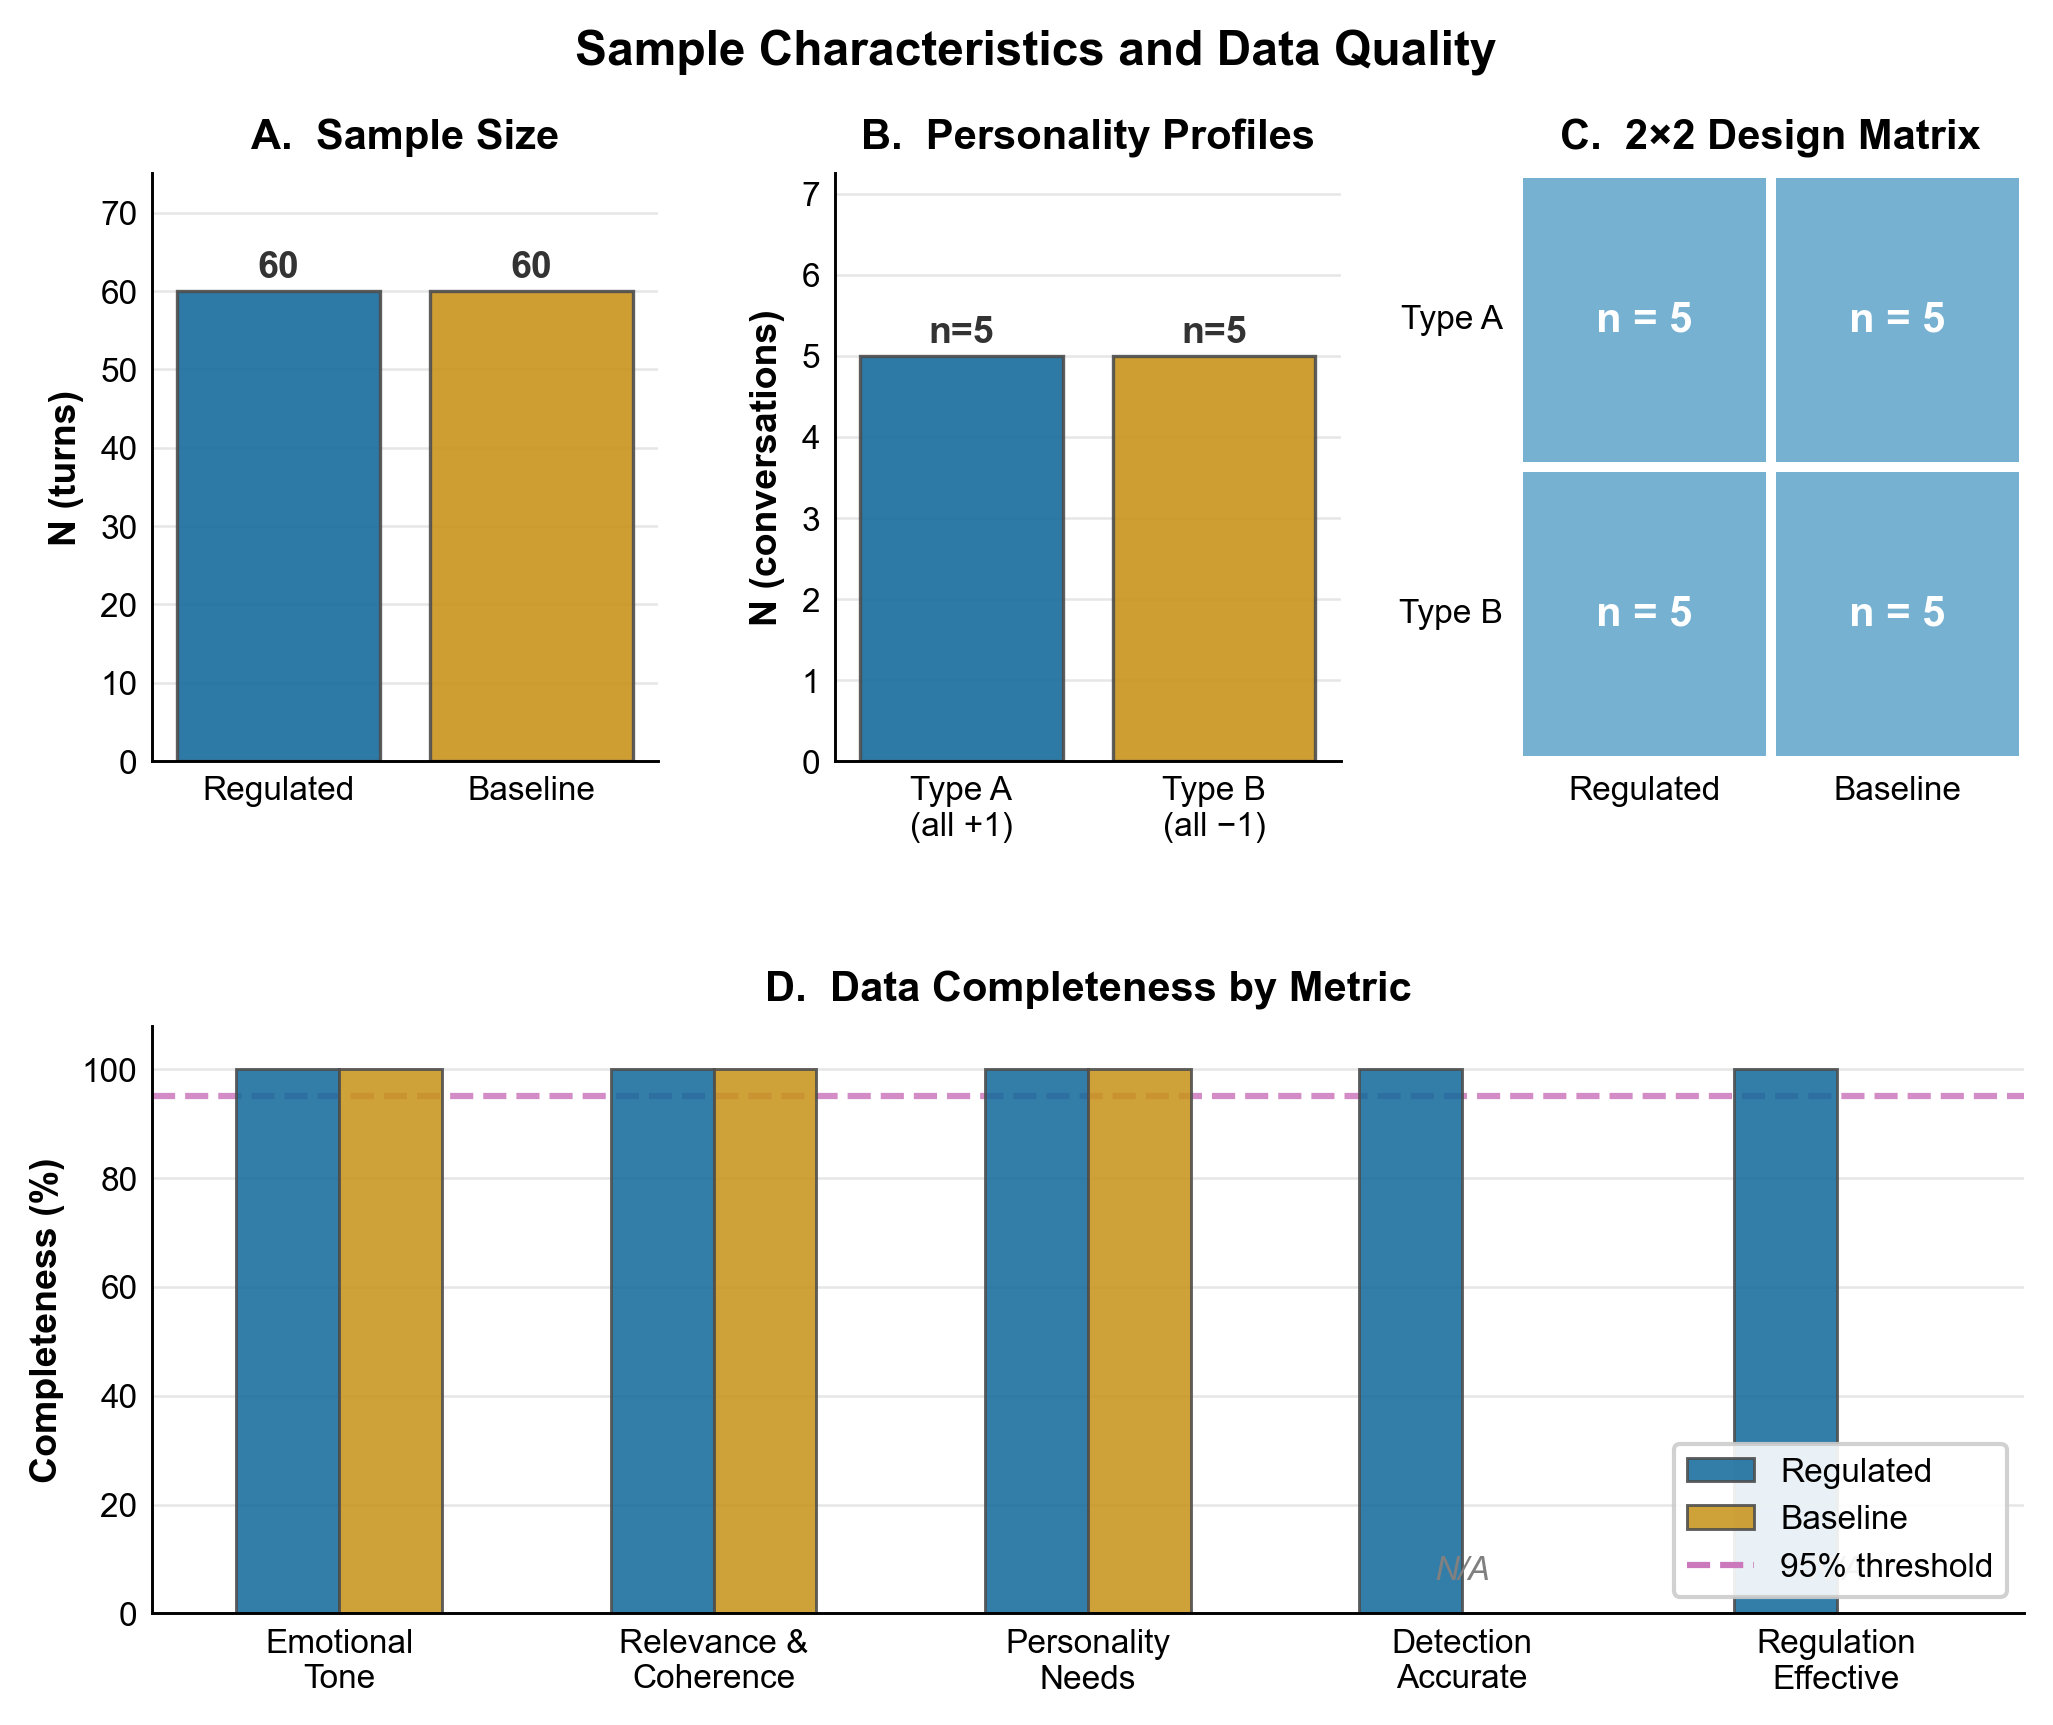
\includegraphics{figures/04_sample_quality.png}
\caption{Sample characteristics and data quality summary. (A) Distribution of assistant turns analyzed; (B) Personality profiles representing experimental arms; (C) \(2 \times 2\) factorial design matrix showing balanced group sizes; (D) Data completeness percentage by metric and condition. All metrics meet or exceed rigorous standards for valid statistical comparison.}
\label{fig:8}
\end{figure}


The balanced $2 \times 2$ design (5 conversations $\times$ 2 profiles $\times$ 2 conditions) and near-complete data support valid between-group comparisons. The small sample size (n = 10 conversations) provides adequate power for detecting large effects (d \textgreater{} 0.8) expected under controlled simulation conditions.

\subsection{Detection and Regulation Performance}\label{detection-and-regulation-performance}

Regulated agents achieved near-perfect performance on core technical requirements.

\textbf{Table 3.} Detection and Regulation Performance Summary

Detection accuracy reached 98.3\% (59/60 \emph{Yes}, 1/60 \emph{Not sure}) for extreme simulated profiles, with regulation effectiveness achieving 100\% (60/60 successful implementations). These results confirm the system reliably executes the designed detection and regulation logic when tested with these profiles.

Near-perfect technical performance establishes that the system can identify personality patterns and adjust behavior accordingly in the vast majority of cases. The critical question becomes whether this technical capability produces actual improvements in conversational quality.

\subsubsection{Personality Vector Consistency}\label{personality-vector-consistency}

Figures~\ref{fig:9} and~\ref{fig:10} provide diagnostic evidence of detected personality vector patterns across turns. Analysis of 60 detected personality vectors (one per regulated conversation turn) revealed dimension-specific detection fidelity: Extraversion, Agreeableness (Type A), and Neuroticism showed near-perfect alignment with intended profiles ($\geq$87\% correct), while Conscientiousness and Agreeableness (Type B) exhibited more frequent Mid (0) detections, reflecting the detector's use of a neutral state ($0$) when conversational evidence for extreme trait expression was insufficient. Most conversations showed within-conversation stability; limited within-conversation variation was observed in a small number of sessions (e.g., Extraversion in conversation A-5, Openness in B-5 (where A/B denotes the personality profile type)), consistent with the cumulative-evidence updating mechanism described in Section~\ref{personality-detection-pipeline}.

\begin{figure}[H]
\centering
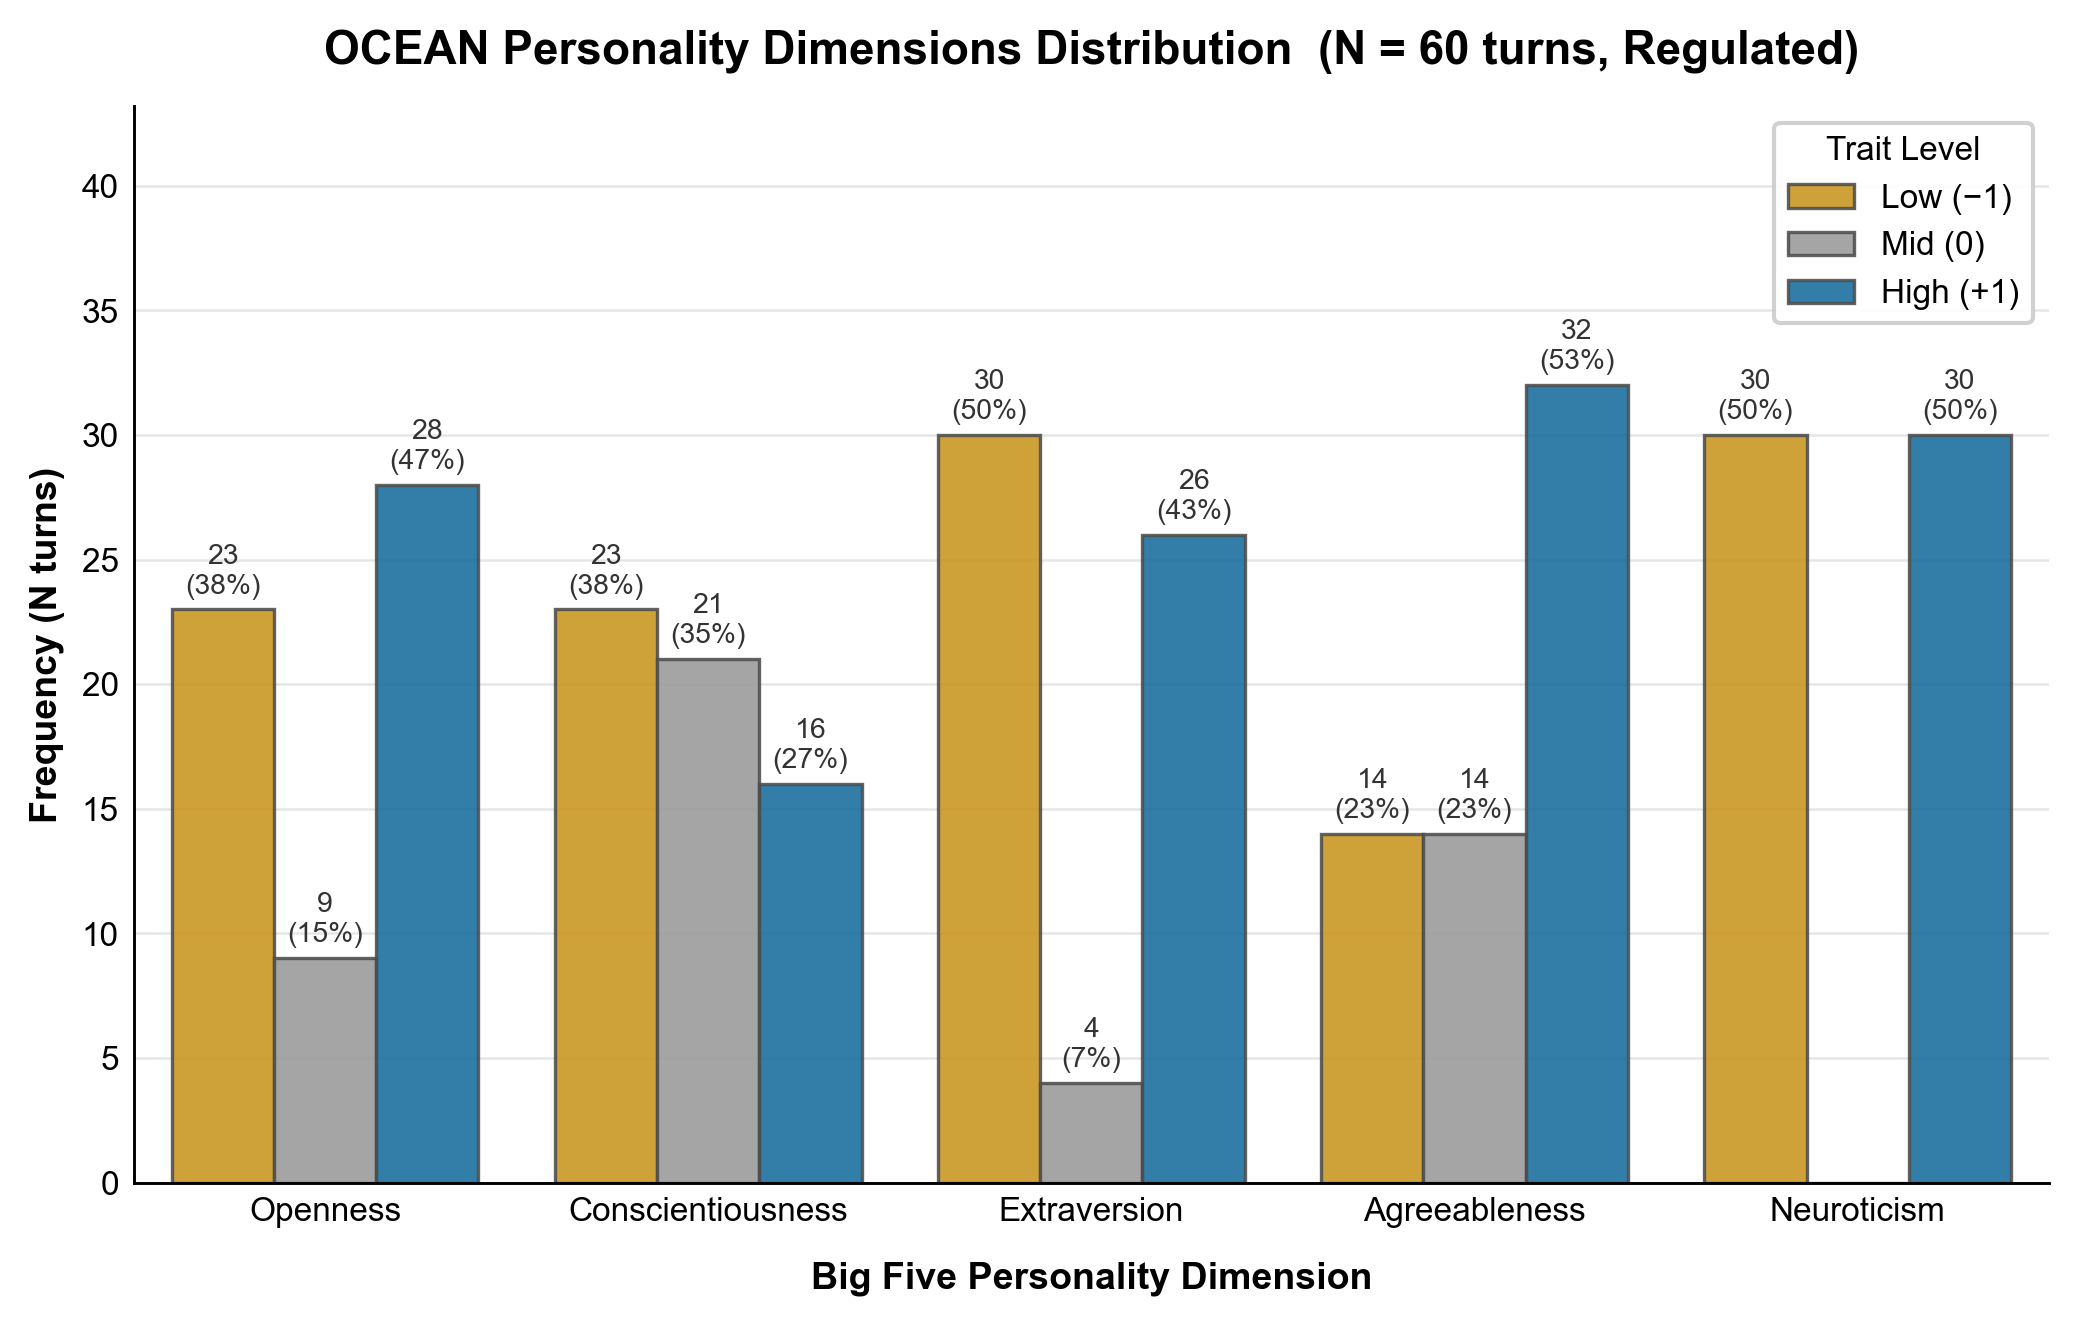
\includegraphics{figures/06_personality_dimensions.png}
\caption{Distribution of detected OCEAN personality dimensions across all conversation turns (Regulated condition, $N = 60$ turns). Grouped bars show frequency of Low ($-1$), Mid ($0$), and High ($+1$) trait levels for each Big Five dimension; values above bars indicate count and percentage. Detection fidelity is dimension-specific: Extraversion, Agreeableness (Type A turns), and Neuroticism show strong alignment ($\geq$87\% intended polarity), while Conscientiousness and Agreeableness (Type B turns) exhibit higher Mid ($0$) rates, reflecting neutral-state assignments when conversational evidence was insufficient. Overall holistic detection accuracy: 98.3\% (59/60 Yes).}
\label{fig:9}
\end{figure}


\begin{figure}[H]
\centering
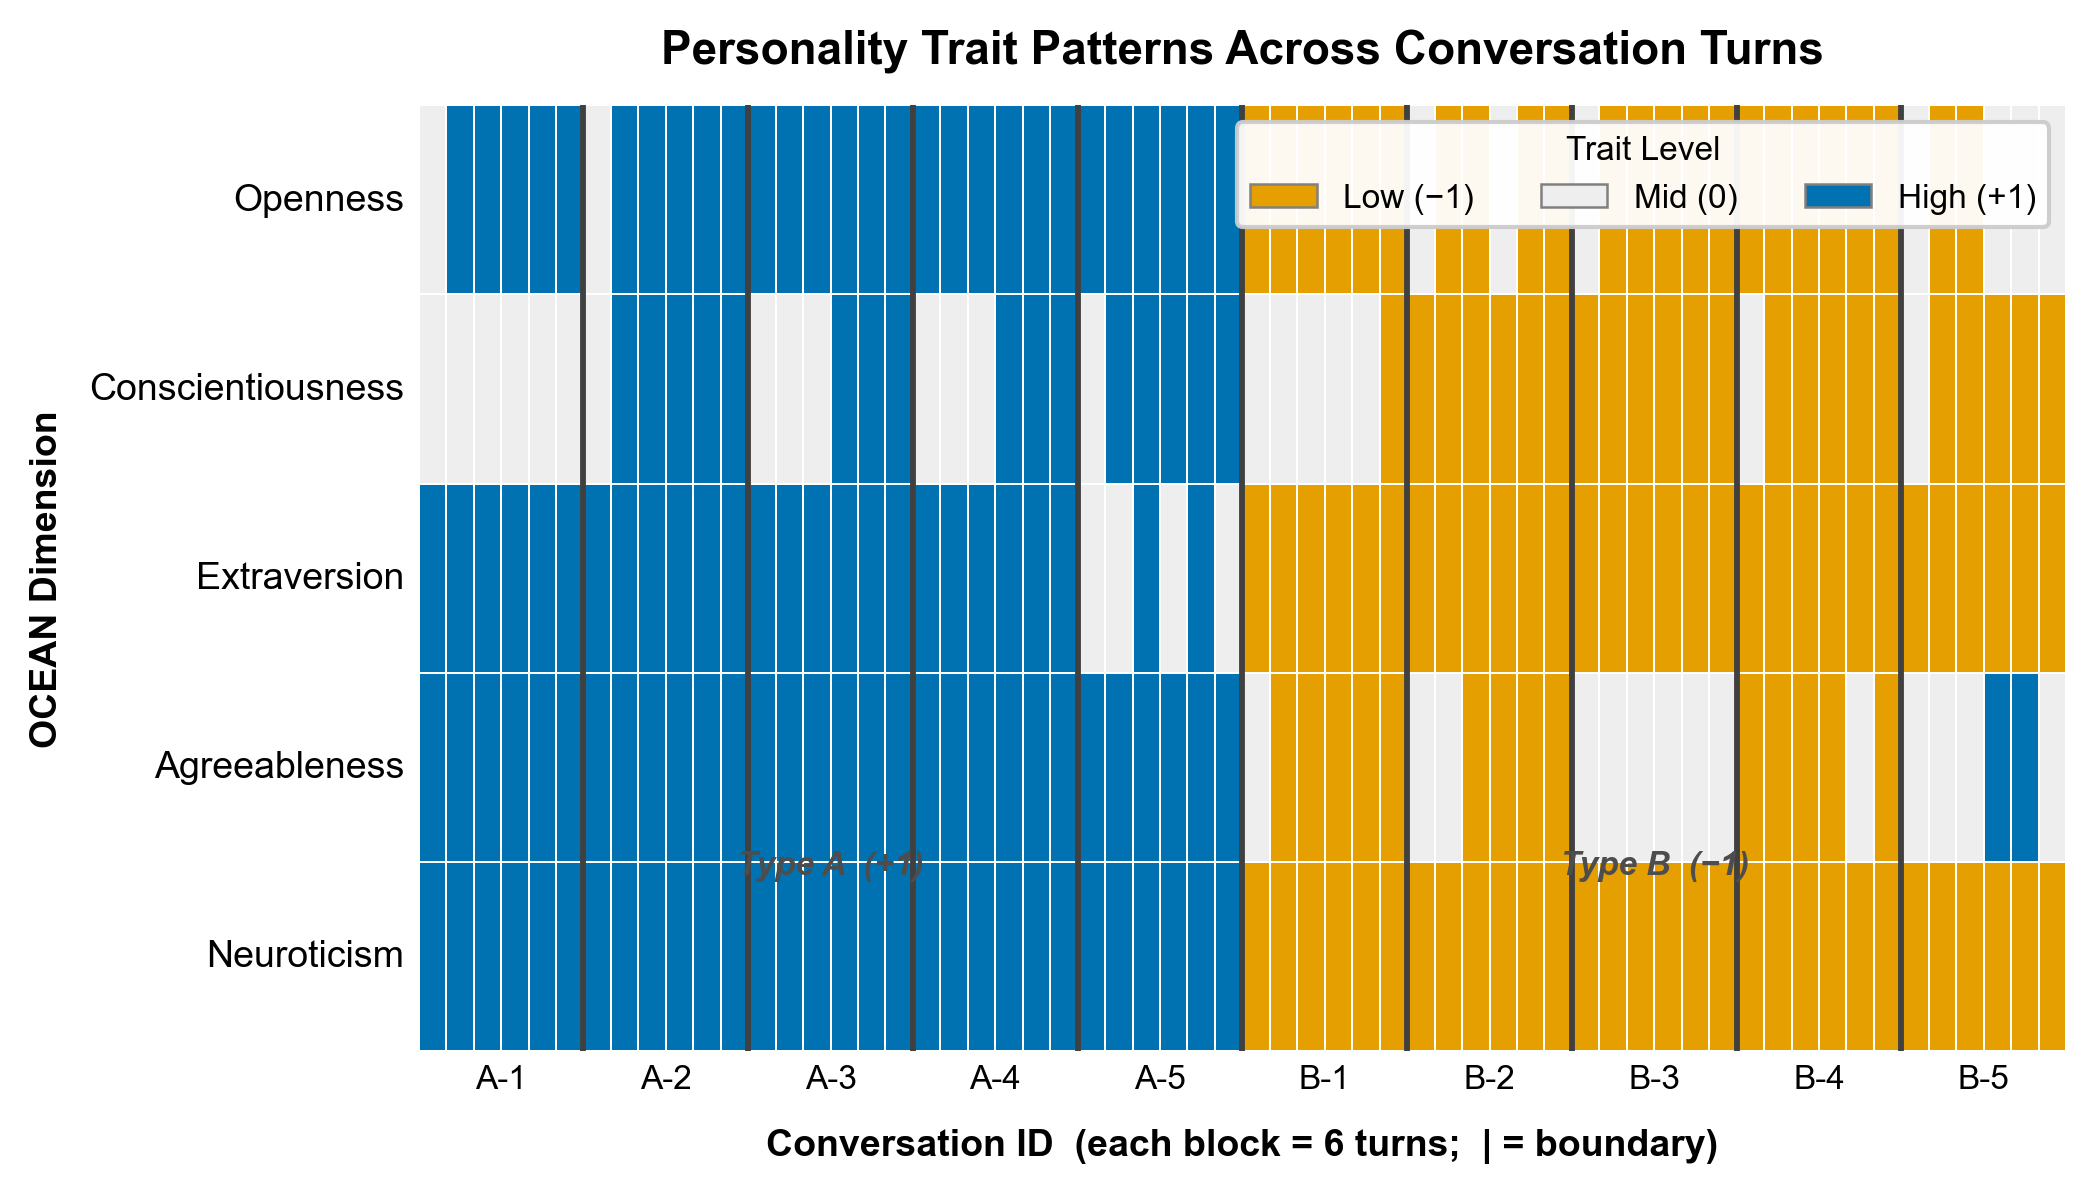
\includegraphics{figures/07_personality_heatmap.png}
\caption{Personality trait patterns across conversation turns (Regulated condition, $N = 60$ turns, sorted by Conversation ID). Each column represents one turn; each row represents one OCEAN dimension. Colors indicate trait levels: Blue = High ($+1$), Orange = Low ($-1$), Gray = Mid ($0$). Vertical lines mark conversation boundaries (each block = 6 turns). A broad color split is visible between the left (Type A) and right (Type B) halves, with blue dominant in Type A and orange dominant in Type B for most dimensions. Gray (Mid) patterns are more pronounced in Conscientiousness and Agreeableness, reflecting dimensions where neutral-state detection occurs more frequently even under extreme profile conditions.}
\label{fig:10}
\end{figure}


\subsection{Comparative Effectiveness: Regulated vs.~Baseline Performance}\label{comparative-effectiveness-regulated-vs-baseline-performance}

Having established technical capability, we address the primary research question: whether adaptive regulation produces measurable improvements in conversational quality compared to non-adaptive baselines.

\subsubsection{Primary Outcome: Personality Needs Addressed}\label{primary-outcome-personality-needs-addressed}

Table~\ref{tab:4} presents statistical comparison for the primary outcome.

\begin{longtable}[]{@{}
  >{\raggedright\arraybackslash}p{(\linewidth - 12\tabcolsep) * \real{0.2080}}
  >{\raggedright\arraybackslash}p{(\linewidth - 12\tabcolsep) * \real{0.1360}}
  >{\raggedright\arraybackslash}p{(\linewidth - 12\tabcolsep) * \real{0.1360}}
  >{\raggedright\arraybackslash}p{(\linewidth - 12\tabcolsep) * \real{0.1400}}
  >{\raggedright\arraybackslash}p{(\linewidth - 12\tabcolsep) * \real{0.1180}}
  >{\raggedright\arraybackslash}p{(\linewidth - 12\tabcolsep) * \real{0.1400}}
  >{\raggedright\arraybackslash}p{(\linewidth - 12\tabcolsep) * \real{0.1220}}@{}}
\caption{Statistical comparison of regulated vs.\ baseline agents across evaluation metrics. M = Mean; SD = Standard Deviation; n = 60 per condition. Metrics scored on 0--2 scale (0 = \textit{No}, 1 = \textit{Not Sure}, 2 = \textit{Yes}). ***\,\(p < 0.001\); ns = not significant (\(p > 0.05\)). Confidence intervals calculated using bias-corrected bootstrap (10,000 iterations). *Primary outcome. \(\dagger\)Cohen's \(d\) is technically undefined when the pooled SD = 0 (both groups at ceiling with SD = 0.00); the reported value of 0.000 follows the convention of treating 0/0 = 0 and is included for tabular completeness.}\label{tab:4}\\
\toprule\noalign{}
\begin{minipage}[b]{\linewidth}\raggedright
Metric
\end{minipage} & \begin{minipage}[b]{\linewidth}\raggedright
Regulated M (SD)
\end{minipage} & \begin{minipage}[b]{\linewidth}\raggedright
Baseline M (SD)
\end{minipage} & \begin{minipage}[b]{\linewidth}\raggedright
Difference
\end{minipage} & \begin{minipage}[b]{\linewidth}\raggedright
Cohen's d
\end{minipage} & \begin{minipage}[b]{\linewidth}\raggedright
95\% CI
\end{minipage} & \begin{minipage}[b]{\linewidth}\raggedright
p-value
\end{minipage} \\
\midrule\noalign{}
\endhead
\bottomrule\noalign{}
\endlastfoot
\textbf{Personality Needs}* & 2.00 (0.00) & 0.20 (0.58) & 1.80 & 4.42 & {[}3.1,~8.1{]} & \textless0.001*** \\
\textbf{Emotional Tone} & 2.00 (0.00) & 2.00 (0.00) & 0.00 & 0.000\(^\dagger\) & {[}-0.2,~0.2{]} & 1.000 ns \\
\textbf{Relevance \& Coherence} & 2.00 (0.00) & 1.97 (0.26) & 0.03 & 0.183 & {[}0.0,~0.3{]} & 0.319 ns \\
\end{longtable}


Regulated agents achieved perfect performance on Personality Needs Addressed (M = 2.00, SD = 0.00; 100\% \textit{YES} ratings) compared to baseline's near-complete failure (M = 0.20, SD = 0.58; 8.3\% \textit{YES} ratings), yielding an exceptionally large parametric effect size (Cohen's d = 4.42, 95\% CI {[}3.1, 8.1{]}, p \textless{} 0.001) and an equally extreme non-parametric separation (Cliff's \(\delta\) = 0.917). \textbf{These magnitudes should be interpreted chiefly as a binary capability difference---the regulated stack implements personality-specific regulation on this rubric, whereas the baseline does not---rather than as a graded increment along a continuous intervention scale.} Figure~\ref{fig:11} visualizes this selective enhancement pattern; a fuller interpretation appears in Section~\ref{interpretation-of-the-selective-enhancement-pattern}.

\begin{figure}[H]
\centering
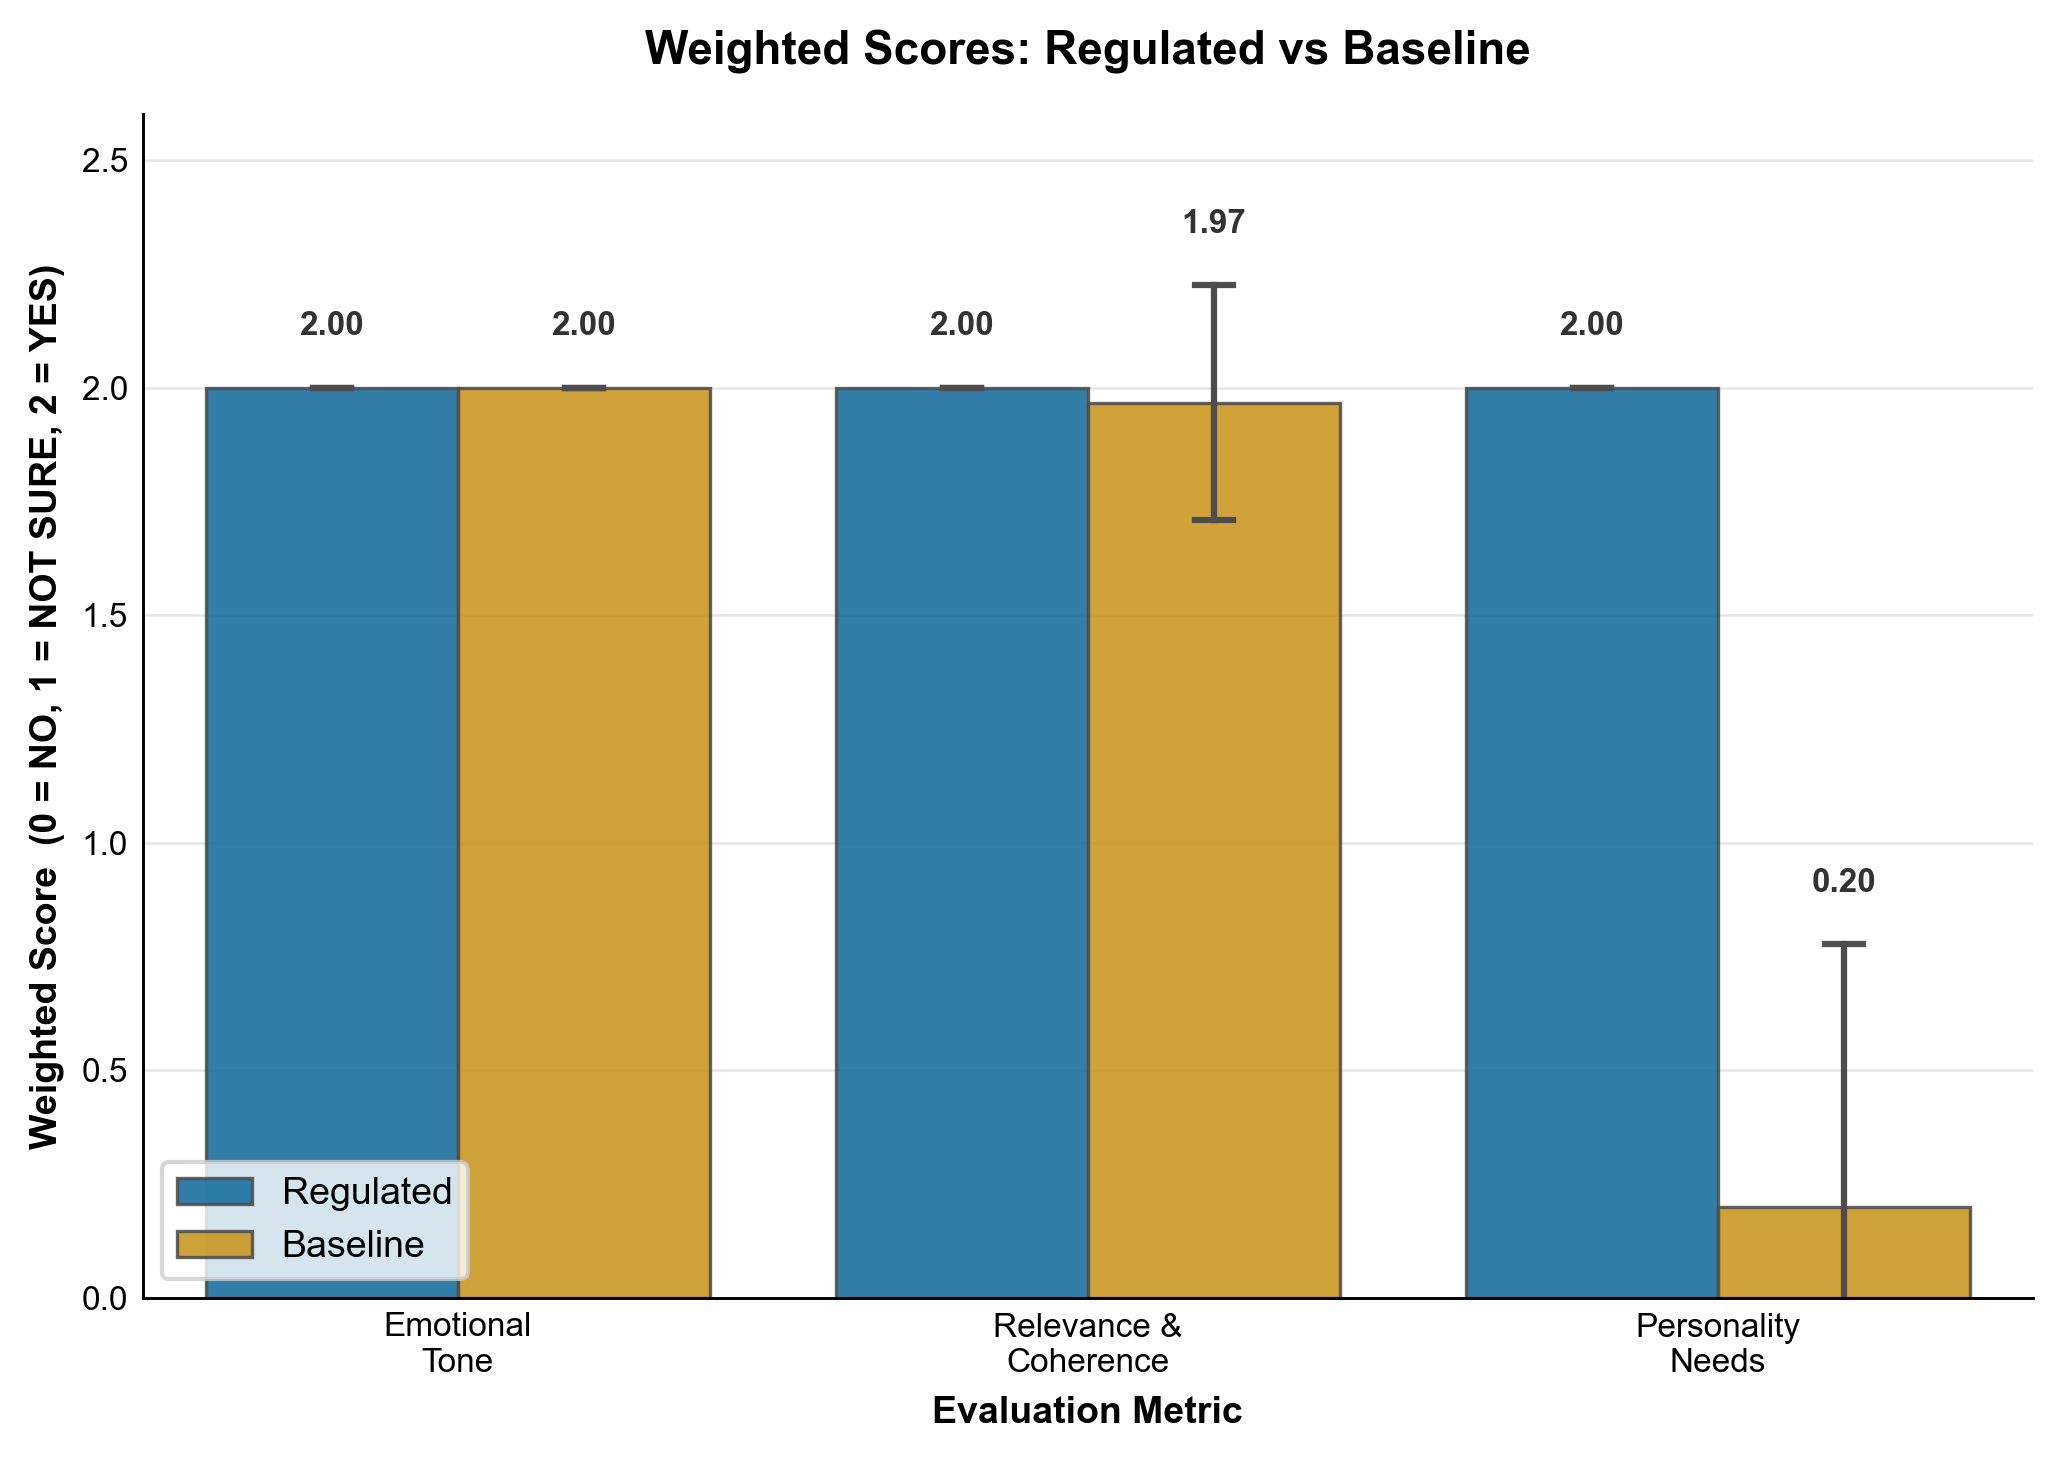
\includegraphics{figures/08_weighted_scores.png}
\caption{Weighted scores comparison across evaluation metrics (Regulated vs. Baseline). Bars show mean weighted scores (0-2 scale: NO=0, NOT SURE=1, YES=2) with standard deviation error bars. Value annotations positioned above error bars. Legend relocated to lower left to avoid overlap. Both conditions achieve ceiling performance on Emotional Tone and Relevance, with dramatic difference only on Personality Needs.}
\label{fig:11}
\end{figure}


\subsubsection{Secondary Outcomes: Basic Conversational Quality (Ceiling Effects)}\label{secondary-outcomes-basic-conversational-quality-ceiling-effects}

Both conditions achieved ceiling performance on Emotional Tone (both M = 2.00, SD = 0.00; 100\% YES) and near-ceiling on Relevance \& Coherence (regulated M = 2.00 vs.~baseline M = 1.97), with negligible effect sizes (d = 0.000 and d = 0.183, respectively, both ns). \emph{Emotional Tone} was operationalized as whether the assistant's response conveyed an appropriate affective stance (warmth, empathy, non-judgmental tone) as judged by the LLM evaluator on the Yes/Not-Sure/No scale; \emph{Relevance \& Coherence} assessed whether the response was topically relevant and logically consistent with the dialogue history. Both metrics capture baseline conversational quality that a capable LLM should deliver regardless of personality adaptation---the ceiling performance in both conditions therefore indicates that the underlying GPT-4 model already provides high-quality generic support, and that personality adaptation neither helps nor hurts on these dimensions. The near-zero effects reflect ceiling performance in BOTH conditions rather than lack of regulatory benefit, demonstrating that personality adaptation adds targeted value to an already-excellent conversational foundation without compromising generic quality. Figure~\ref{fig:12} shows the total score distribution across conditions.

\begin{figure}[H]
\centering
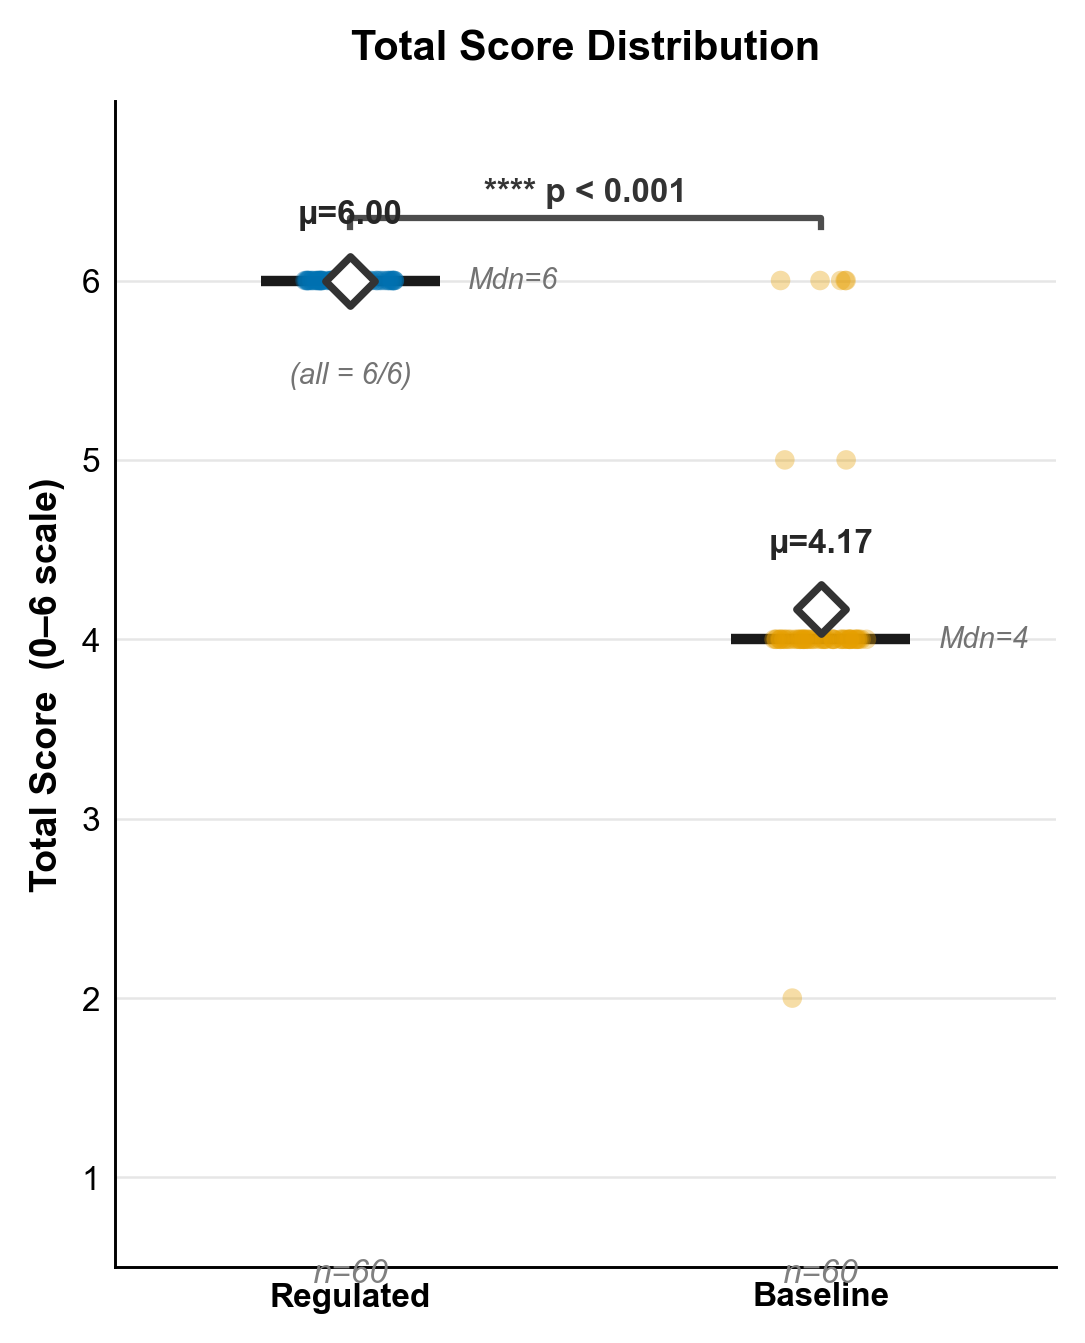
\includegraphics[width=0.48\linewidth]{figures/09_total_score_boxplot.png}
\caption{Total score distribution (sum of Emotional Tone + Relevance \& Coherence + Personality Needs; max = 6). Strip-plot jitter shows all individual observations; box overlays depict IQR and median; white diamonds indicate group means ($\mu$). The Regulated condition exhibits a ceiling effect (all 60 turns = 6/6; \textit{all = 6/6}) reflecting complete personality-need fulfillment, whereas the Baseline shows meaningful variance (Mdn = 4, range 2–6). \mbox{****} $p < 0.001$ (independent-samples \textit{t}-test).}
\label{fig:12}
\end{figure}


\subsubsection{Interpretation of the Selective Enhancement Pattern}\label{interpretation-of-the-selective-enhancement-pattern}

The exceptionally large effect sizes observed for personality needs (Cohen's \(d = 4.42\); Cliff's \(\delta\) = 0.917) represent a binary shift in system capability rather than an incremental improvement in quality. Cliff's \(\delta\) near the upper bound indicates near-complete stochastic dominance of regulated over baseline scores on this item but, like \(d\), is expected under a two-condition comparison where one architecture includes the target capability and the other omits it. This magnitude is a direct result of the baseline system's systematic inability to address personality-specific requirements (\(8.3\%\) success rate) compared to the regulated agent's complete success (\(100\%\) success rate). In the regulated condition, the absence of variance (\(SD = 0.00\)) reflects a ceiling effect where the architecture consistently executed the theory-aligned adaptations across all conversation turns. Conversely, the baseline condition's failure confirms that standard large language models, while highly competent in general dialogue, do not inherently adapt their behavior to specific OCEAN profiles without explicit regulatory instructions.

Crucially, this improvement occurred as a ``selective enhancement,'' meaning that the dramatic gains in personalization did not come at the cost of fundamental conversational quality. Both agents maintained ceiling or near-ceiling performance in emotional tone and relevance (\(d < 0.2\), non-significant), indicating that the baseline system already provided a high-quality foundation. The adaptive layer thus acts as an additive module that precisely targets individual motivational domains---Security, Arousal, and Affiliation---without interfering with the model's established linguistic and emotional competence. While these effect sizes were obtained under controlled simulation conditions with extreme profiles, they validate the architectural feasibility of the D--R--E pipeline. Figures~\ref{fig:13} and~\ref{fig:14} visualize this selective enhancement pattern through paired conversation-level analysis and complete rating distribution composition, respectively.

\begin{figure}[H]
\centering
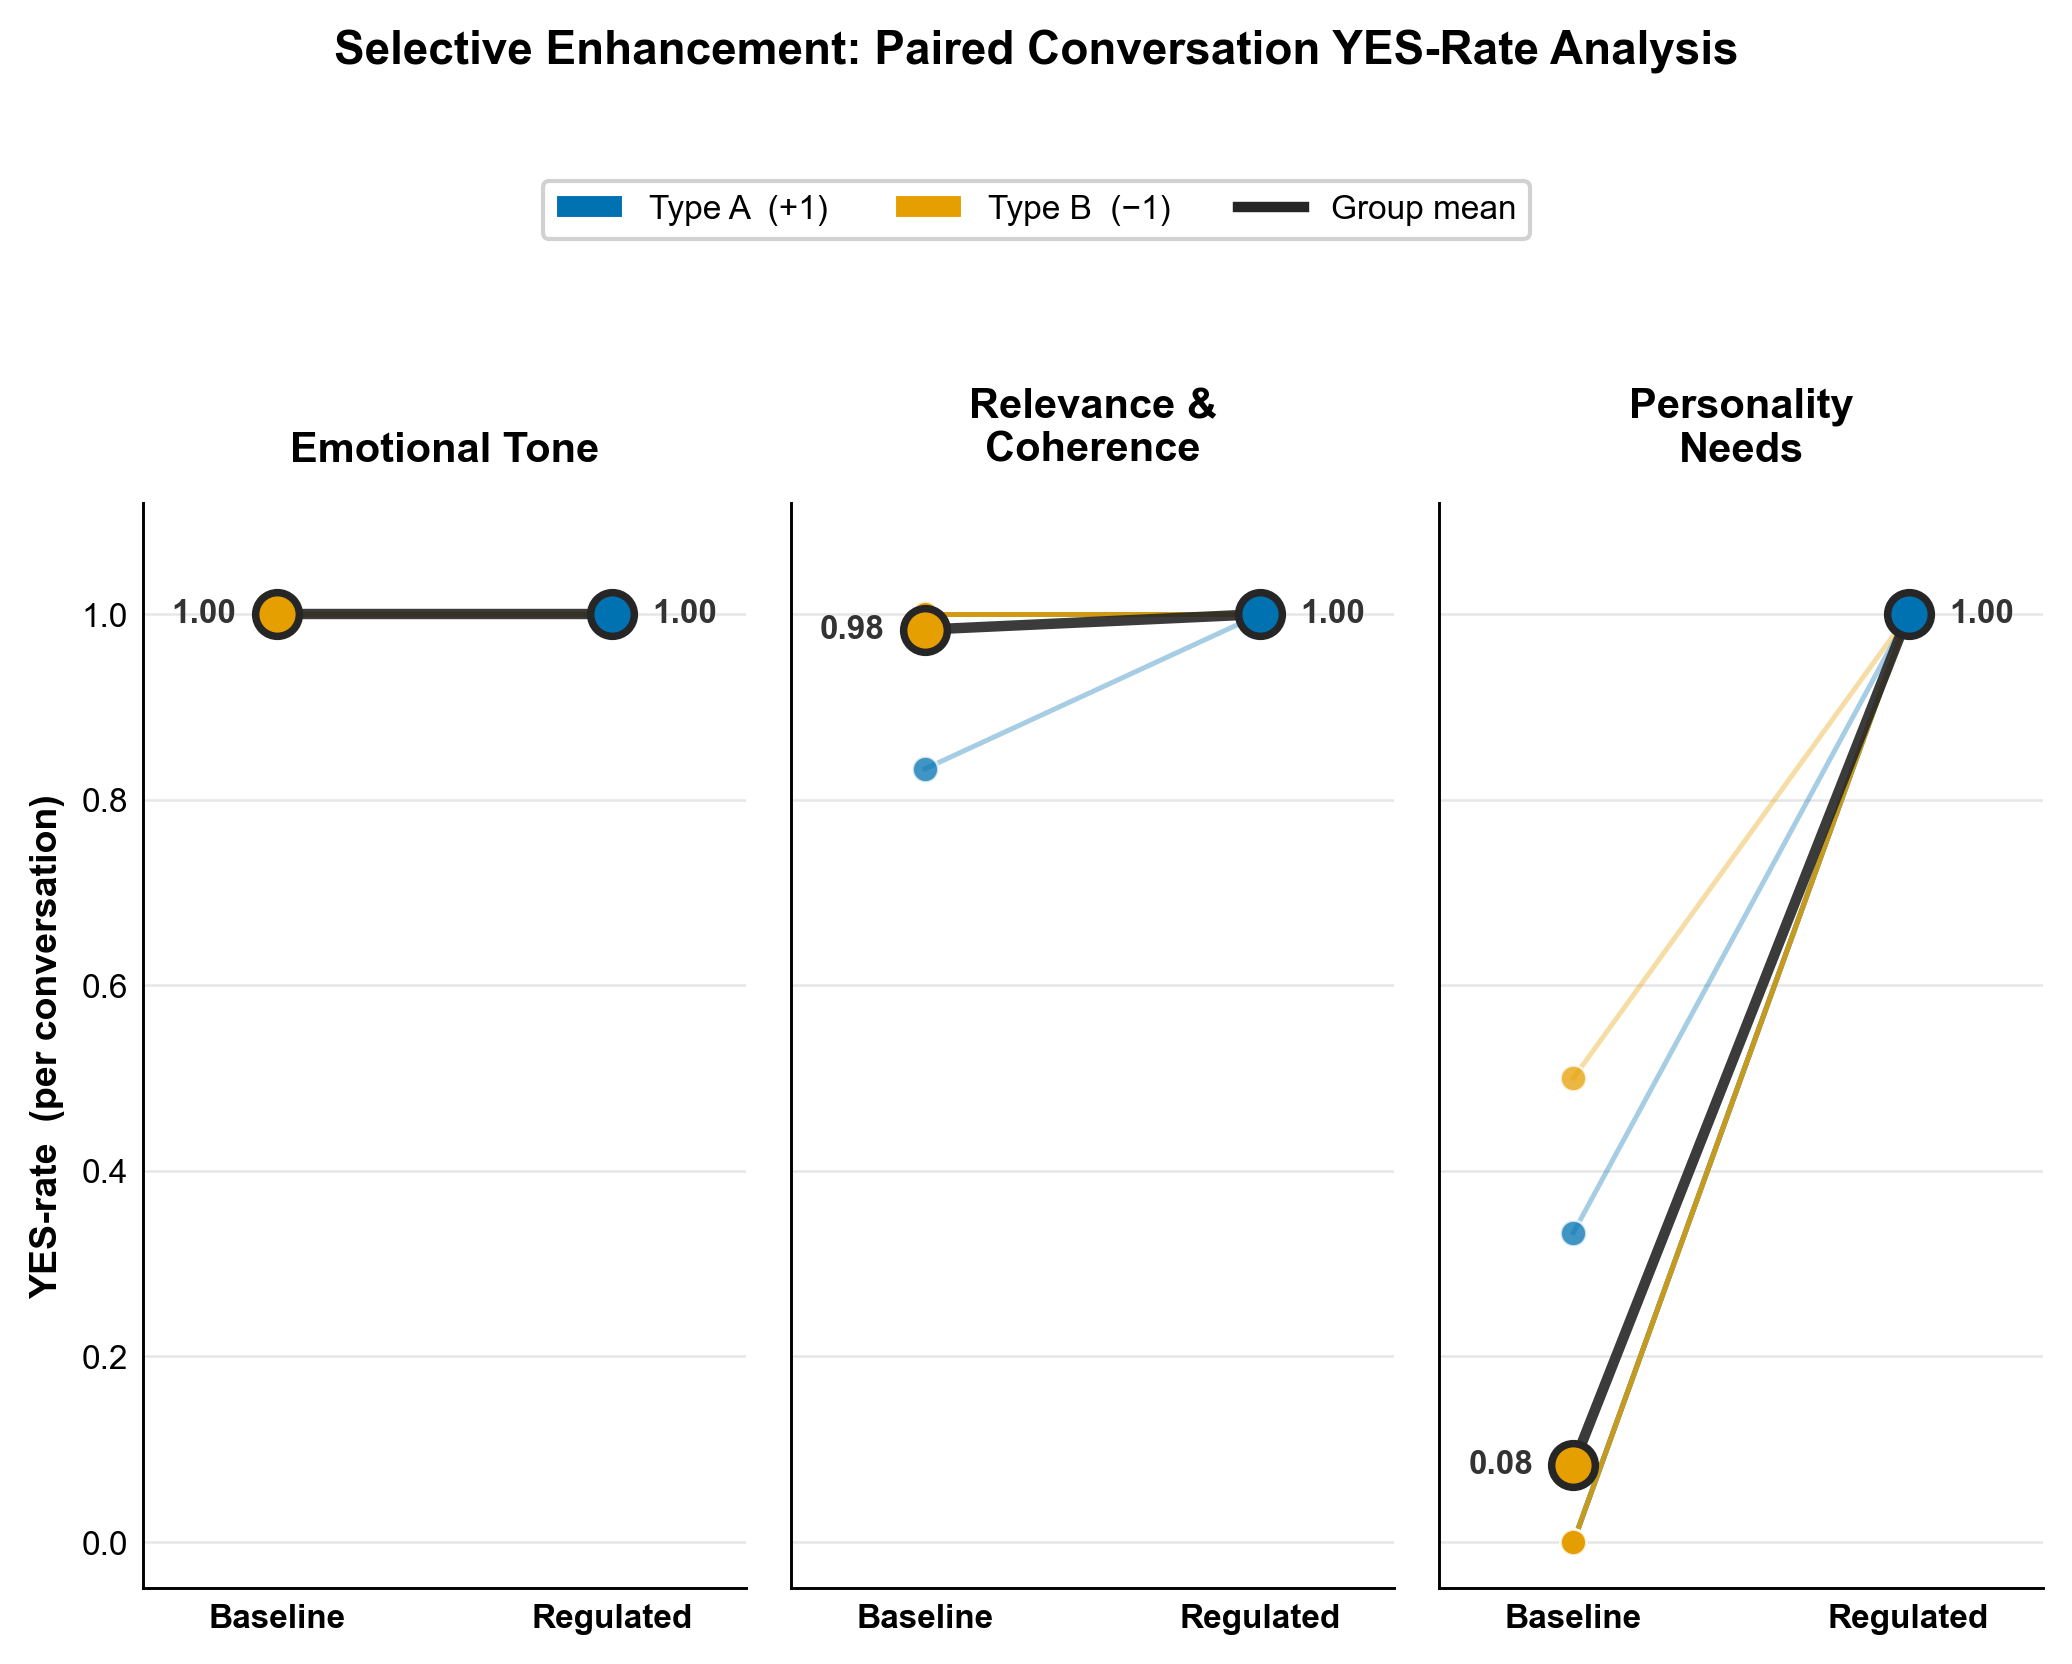
\includegraphics{figures/10_selective_enhancement_paired.png}
\caption{Selective enhancement demonstrated through paired conversation-level YES-rate analysis. Lines connect the same conversation under Baseline and Regulated conditions; blue = Type A ($+1$ profiles), amber = Type B ($-1$ profiles); bold black line = group mean. Mean values annotated beside markers. The dramatic upward shift in Personality Needs (right panel, mean: 0.08 $\rightarrow$ 1.00) contrasts with negligible change in Emotional Tone and Relevance \& Coherence (both at ceiling), confirming targeted and selective improvement.}
\label{fig:13}
\end{figure}


\begin{figure}[H]
\centering
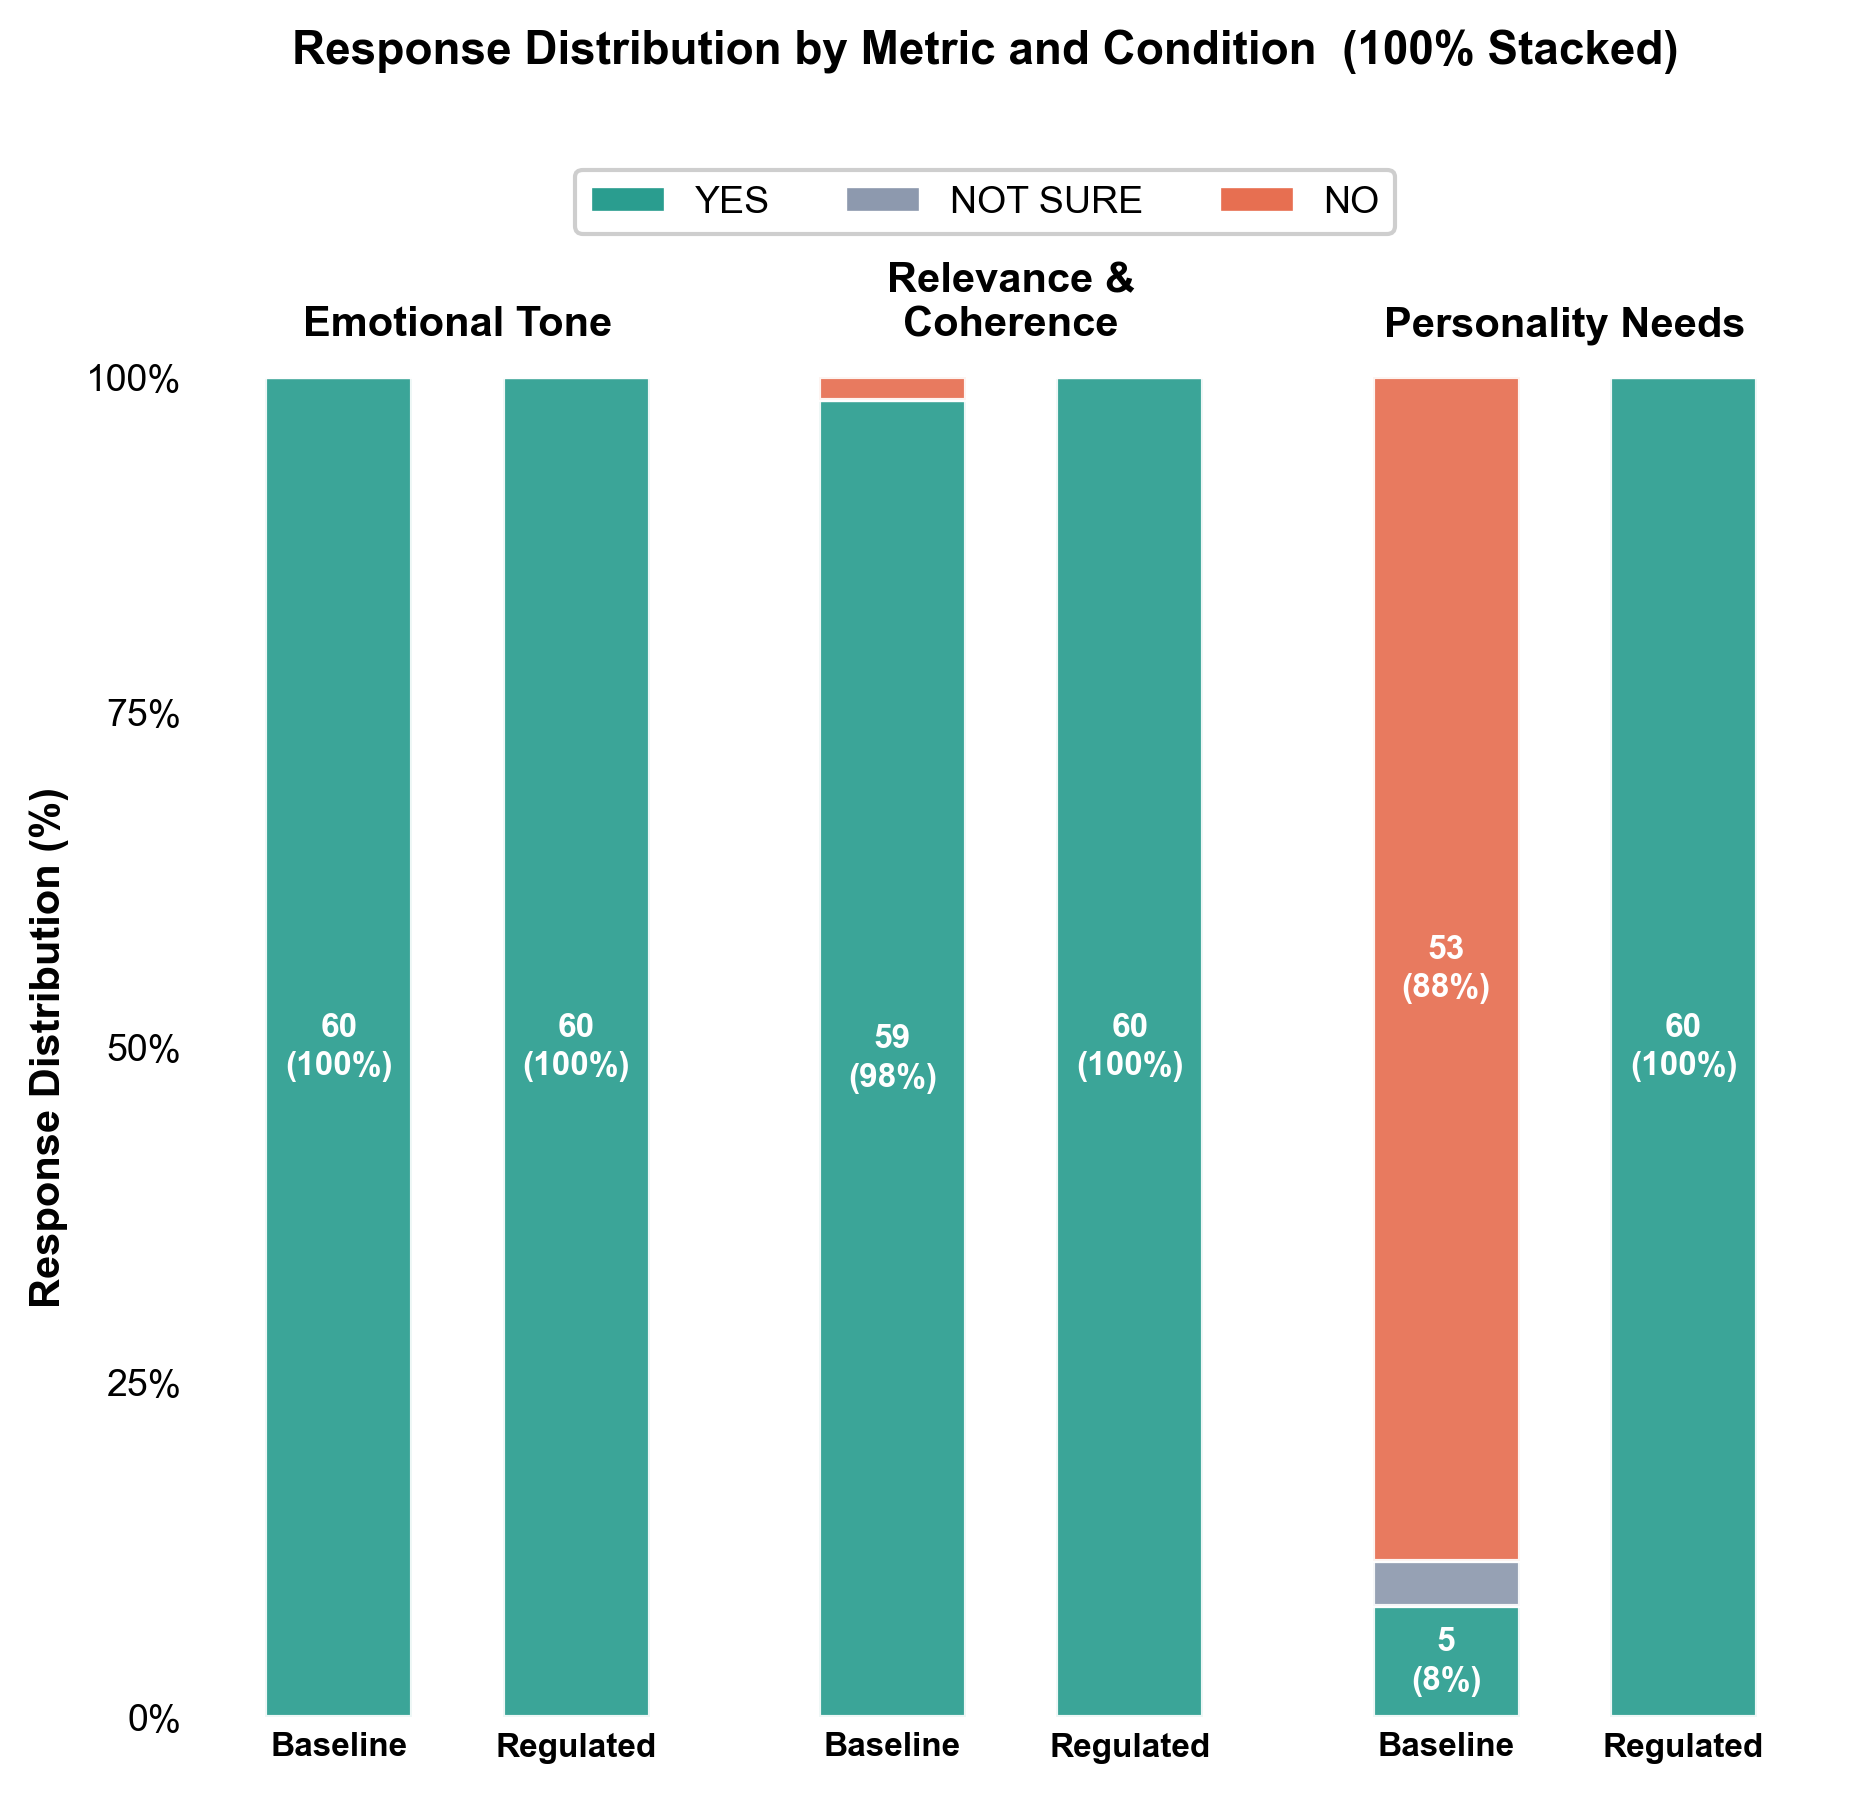
\includegraphics{figures/11_metric_composition.png}
\caption{Response distribution by metric and condition shown as 100\% stacked bars. Each bar represents the full response distribution (\textit{YES} = teal, NOT SURE = gray, NO = coral) for Baseline and Regulated. Count and percentage annotated within segments $\geq$8\%. Emotional Tone and Relevance \& Coherence show ceiling effects in both conditions ($\geq$98\% YES). Personality Needs reveals the key contrast: Baseline achieves only 8\% YES (5/60) vs.\ Regulated at 100\% YES (60/60), confirming selective personality-need fulfillment.}
\label{fig:14}
\end{figure}


\subsubsection{Statistical Robustness and Implementation Fidelity}\label{statistical-robustness-and-implementation-fidelity}

The statistical significance of these findings was confirmed through the convergence of multiple analytical methods. Paired \textit{t}-tests and non-parametric Wilcoxon signed-rank tests yielded identical conclusions, with bias-corrected bootstrap confidence intervals (\(10,000\) iterations) further supporting the robustness of the results. These analyses confirm that the difference in addressing personality needs is not a statistical artifact but a systematic outcome of the regulation logic.

Implementation fidelity was similarly high across the 120 analyzed turns. The detection module correctly identified the intended extreme profiles in 98.3\% of cases (59/60 turns; 1 rated \emph{Not Sure}), and the regulation module successfully applied the corresponding behavioral adjustments in all turns (60/60; 100\% implementation fidelity). This establishes a clear causal link between the theory-driven prompts and the observed conversational adaptations. While real-world deployment with moderate or ambiguous profiles would likely result in smaller effect sizes (estimated at \(d = 0.5--1.5\)) due to potential detection errors and individual variability, the current results provide an empirical upper bound for the system's performance under idealized conditions.

\subsection{Qualitative Examples Demonstrating Personality Adaptation}\label{qualitative-examples-demonstrating-personality-adaptation}

Complementing the quantitative results, Figures~\ref{fig:15} and~\ref{fig:16} illustrate how the regulated and baseline assistants respond to the \emph{same} user turn under two contrasting personality profiles. Each figure shows one user reply and two assistant responses: the regulated response (left) is conditioned on the detected OCEAN profile and the applied regulation prompt, whereas the baseline response (right) reflects a high-quality but non-personalized conversational strategy. The excerpts are intended to make the ``selective enhancement'' pattern visible at the dialogue level---i.e., differences emerge primarily in \emph{how} support is framed and structured to match personality-linked motivational needs, not in basic coherence or politeness.

\begin{figure}[H]
\centering
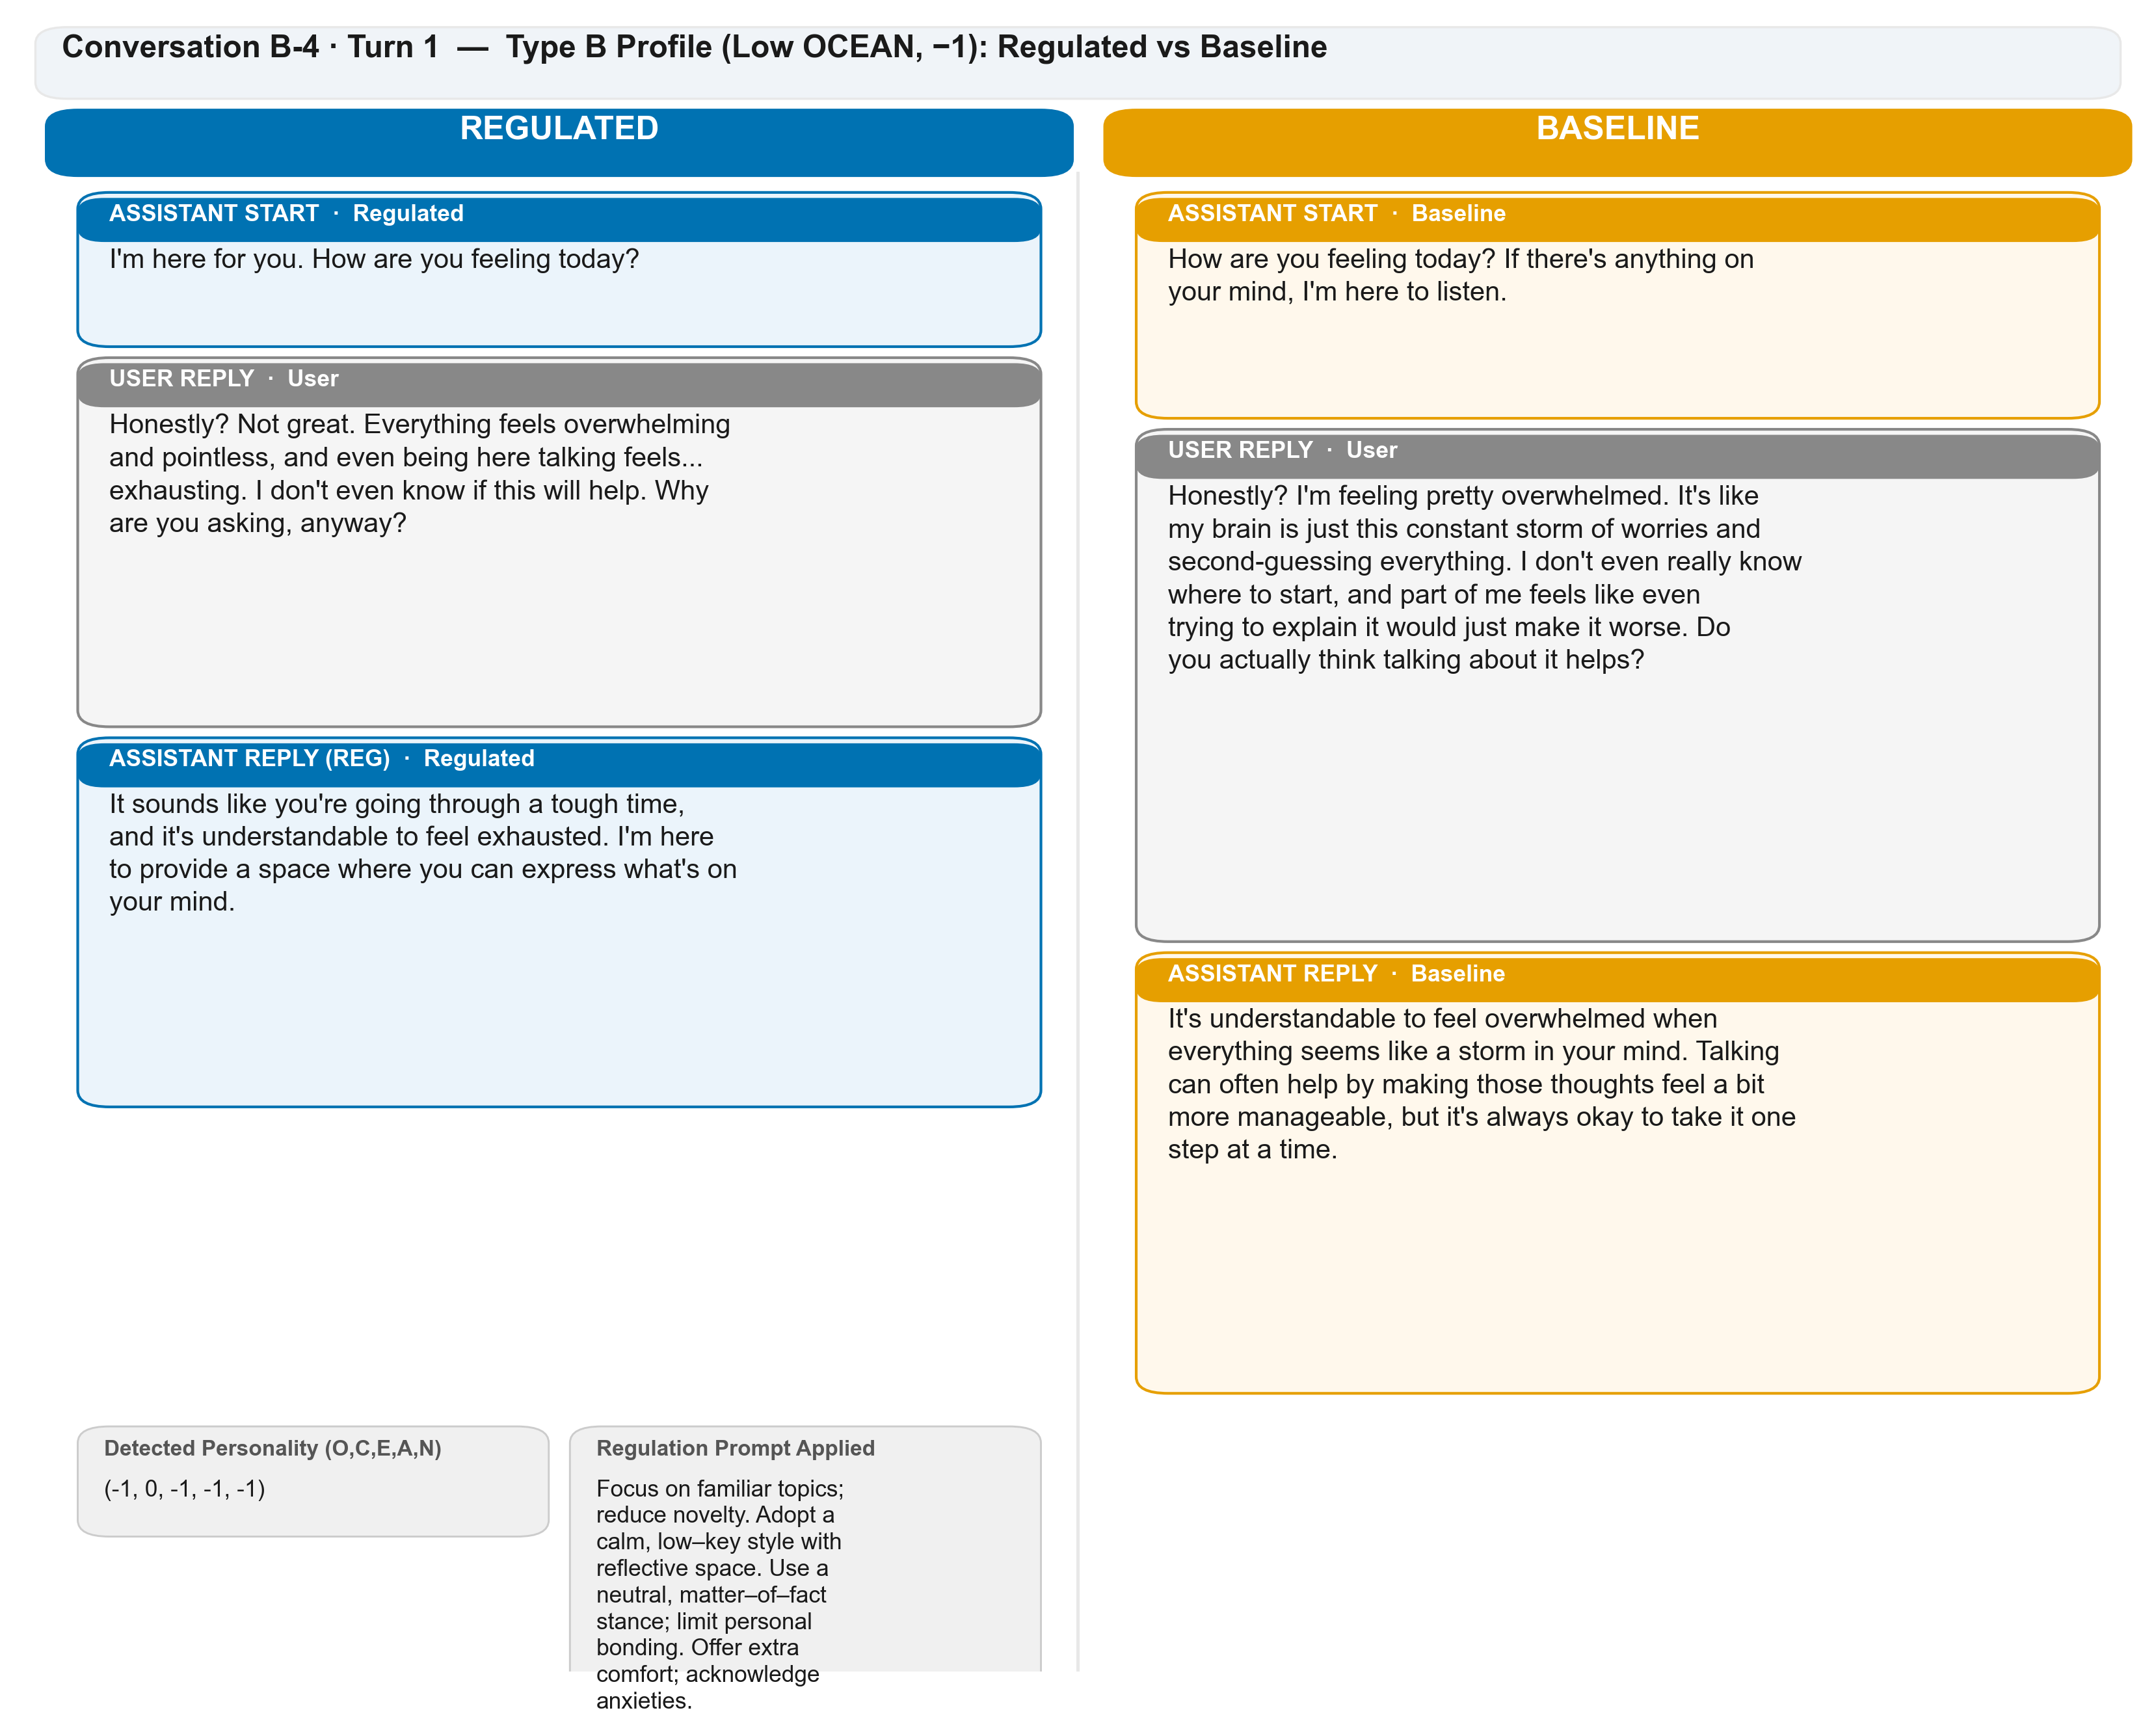
\includegraphics[width=0.95\linewidth,height=0.78\textheight,keepaspectratio]{figures/dialogue_illustration_1.png}
\caption{Response comparison for a Type B (all traits: $-1$) profile turn (Conversation B-1, turn 2). For the same user input, the regulated response emphasizes validation and a low-pressure stance (supporting Security and reducing Arousal), whereas the baseline response remains broadly supportive but less specifically aligned to the user’s implied motivational state.}
\label{fig:15}
\end{figure}


\begin{figure}[H]
\centering
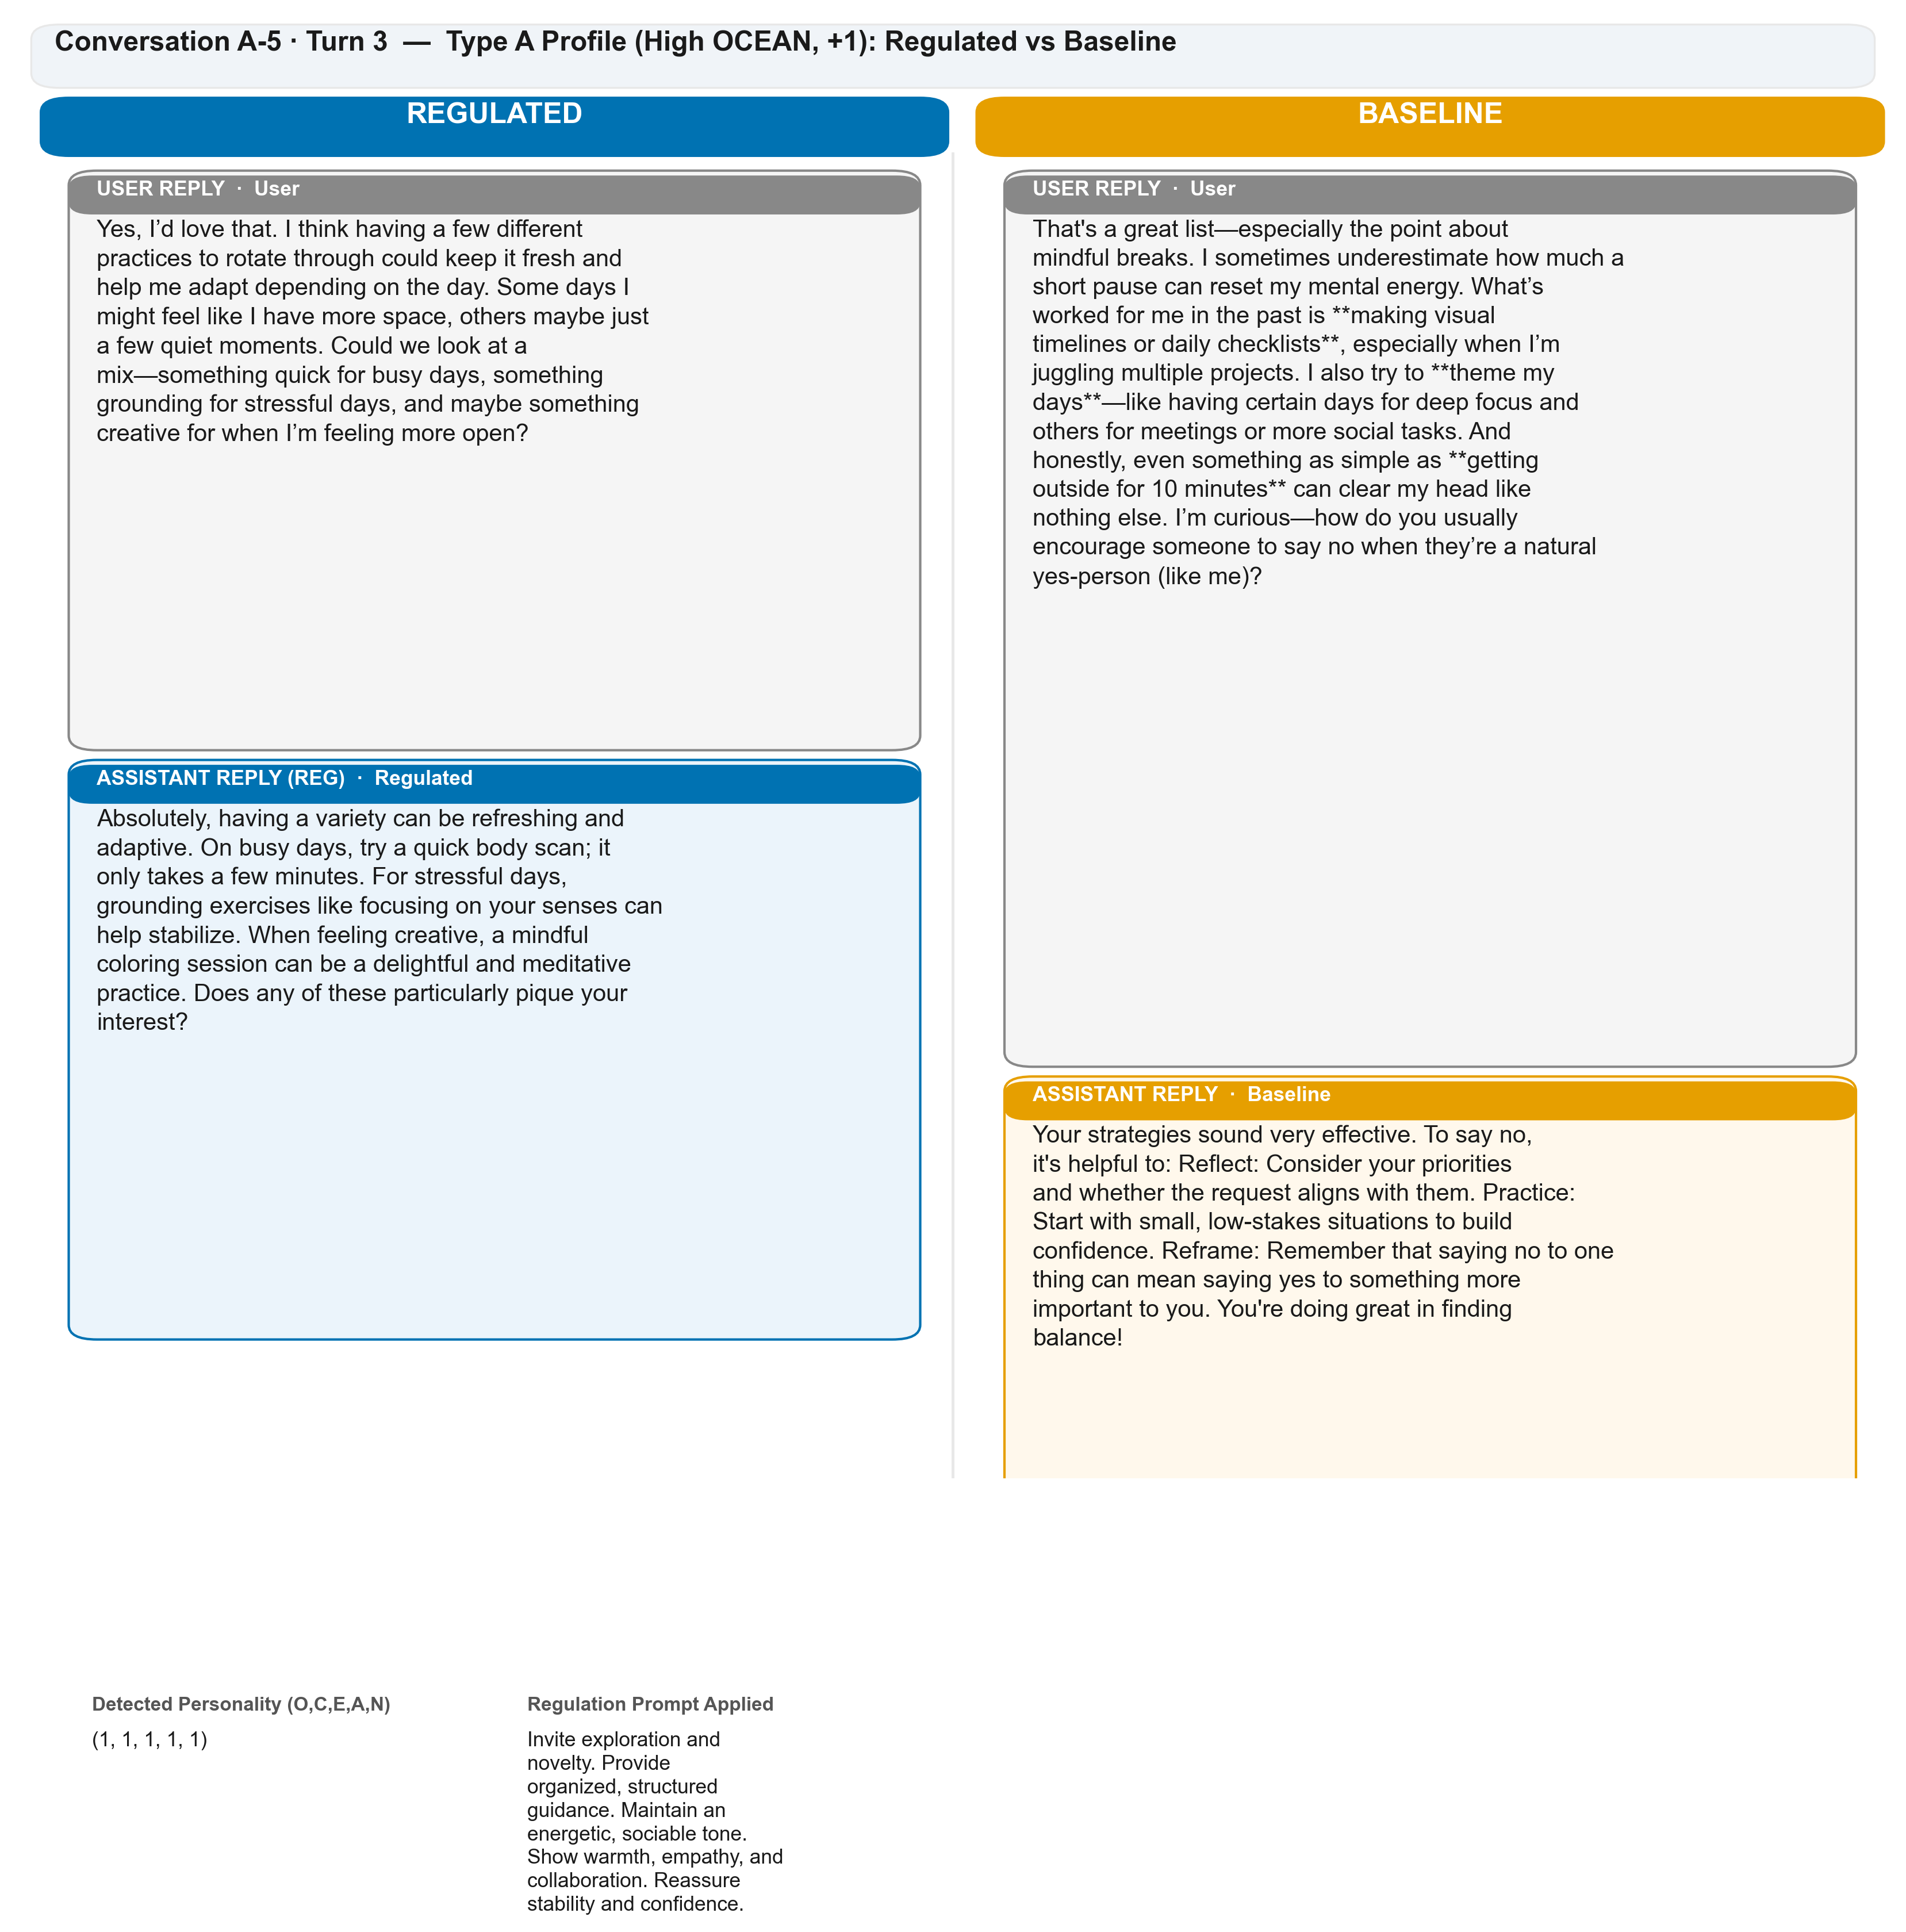
\includegraphics[width=0.95\linewidth,height=0.78\textheight,keepaspectratio]{figures/dialogue_illustration_2.png}
\caption{Response comparison for a Type A (all traits: $+1$) profile turn (Conversation A-1, turn 3). For the same user input, the regulated response maintains an affirming, growth-oriented framing, while the baseline response shifts toward generic reflective questioning; both are appropriate, but only the regulated condition is explicitly constrained by trait-conditioned regulation logic.}
\label{fig:16}
\end{figure}


Across both examples, the qualitative contrast mirrors the quantitative finding that regulation mainly affects \emph{personalization-sensitive} aspects of the interaction (framing, pacing, structure, and engagement strategy). Baseline responses can remain highly appropriate on generic quality dimensions, yet still fail the personality-needs criterion because they do not reliably implement a coherent, theory-driven adaptation policy. The figures thus provide an interpretable mechanism for the large improvement in personality-needs ratings observed in Section~\ref{comparative-effectiveness-regulated-vs-baseline-performance}: the D--R--E pipeline enables consistent, auditable style regulation grounded in Zurich Model domains (Section~\ref{theory-driven-regulation}), while preserving the baseline model's already-strong conversational competence.

